\section{Improving sequential version}
When parallel version can't be improved any more, if you still want to increase the performance you have to review everything about your code, beginning from the basis, the sequential code. In this section we present an improved sequential version from which we will parallelize the code, expecting better performance results.

First of all we did a performance comparison between sequential versions. The first version is called sieve1-seq, and the improved version sieve2-seq.

\begin{table}[h!]
\begin{tabular}{|l|l|l|}
\hline
Version/Block size             & Execution time & Speed-up wrt. sieve1-seq \\ \hline
sieve1-seq 100000000           & 5.298          & 1                        \\ \hline
sieve2-seq 100000000 100000000 & 3.011          & 1.759                    \\ \hline
sieve2-seq 100000000 10000000  & 1.359          & 3.898                    \\ \hline
sieve2-seq 100000000 1000000   & 1.156          & 4.583                    \\ \hline
sieve2-seq 100000000 100000    & 0.861          & 6.153                    \\ \hline
sieve2-seq 100000000 10000     & 1.487          & 3.563                    \\ \hline
sieve2-seq 100000000 1000      & 7.717          & -                        \\ \hline
\end{tabular}
\end{table}

Just improving the sequential version, with no parallelization we achieve an speedup of 6.

\subsection{Worksharing constructs parallelization}
The parallelization of the improved version is simpler as the scheme of the code is more clear now. As we divide sieve of slices, distributing the slices among threads is a clean approach. 

\begin{lstlisting}[caption={Parallelization scheme using worksharing constructs}, captionpos=b]
  #pragma omp parallel for schedule(auto) reduction(+:found)
  for (int from = 2; from <= lastNumber; from += sliceSize) {
    int to = from + sliceSize;
    if (to > lastNumber) to = lastNumber;
    found += eratosthenesBlock(from, to);
  }
\end{lstlisting}
\justify
The following pragma leads to correct code, declaring the parallel region as the main loop of the algorithm, setting schedule to auto as seen in previous sections it seems to work out good, and adding the reduction of the found variable.

\subsection{Task based parallelization}
For this parallelization scheme, we follow the same approach as the worksharing constructs scheme, but we will need to implement manually the reduction, as seen in the previous sections, obtaining the following code. Notice that no granularity has been set, this is because we will analyse which is the propper one.

\begin{lstlisting}[caption={Parallelization scheme task based using manual reduction}, captionpos=b]
  #pragma omp parallel
  #pragma omp single
  {
  int nt = omp_get_num_threads();
  int *found_ac = malloc(sizeof(int)*nt);

  #pragma omp taskloop
  for (int from = 2; from <= lastNumber; from += sliceSize) {
    int to = from + sliceSize;
    if (to > lastNumber) to = lastNumber;
    found_ac[omp_get_thread_num()] += eratosthenesBlock(from, to);
  }

  for(int i = 0; i < nt; i++) found += found_ac[i];
\end{lstlisting}

\subsubsection*{Granularity analysis}
For finding the appropriate granularity with the objective of finding a good balance between correct load balance and less work distribution overhead i tested some values. Here are the results with N=1000000000 and 8 threads.

\begin{table}[h!]
\begin{tabular}{|l|l|}
\hline
Version           & Time (seconds) \\ \hline
grainsize(100)    & 1.44           \\ \hline
num\_tasks(16*nt) & 1.490          \\ \hline
num\_tasks(8*nt)  & 1.512          \\ \hline
default           & 1.564          \\ \hline
num\_tasks(4*nt)  & 1.583          \\ \hline
num\_tasks(2*nt)  & 1.648          \\ \hline
\end{tabular}
\end{table}
\justify
We can see that the value around 16 times the number of threads is fine, the grainsize(100) is the best performing but as it is not depending on the number of threads I prefer the num\_tasks(16*nt) as its value depends on the number of threads.

\subsection{Performance evaluation}
\justify
For this two newer versions I obtained strong scallability plots for both versions.
\justify
The first one corresponds to the worksharing constructs approach. We can observe that the scallability plots are similar at the previous versions, this means we are not loosing scallability while maintaining the speedup to the other versions.
\clearpage
\begin{figure}[!h]
    \centering
    \includegraphics[width=0.9\textwidth]{strongFOR-s2.png}
    \caption{Strong scallability plot for worksharing constructs based approach}
\end{figure}

\justify
Finally, for the task based model it weren't possible to take the graph due to the script is not working with that version. 

\justify
For a final conclusion I measured the execution time with N=100000000 and 1,2,4,8,12 processors and setting the slice size to the optimum found at the begining of this section, 100000 with both versions with the purpose of doing a final comparison.

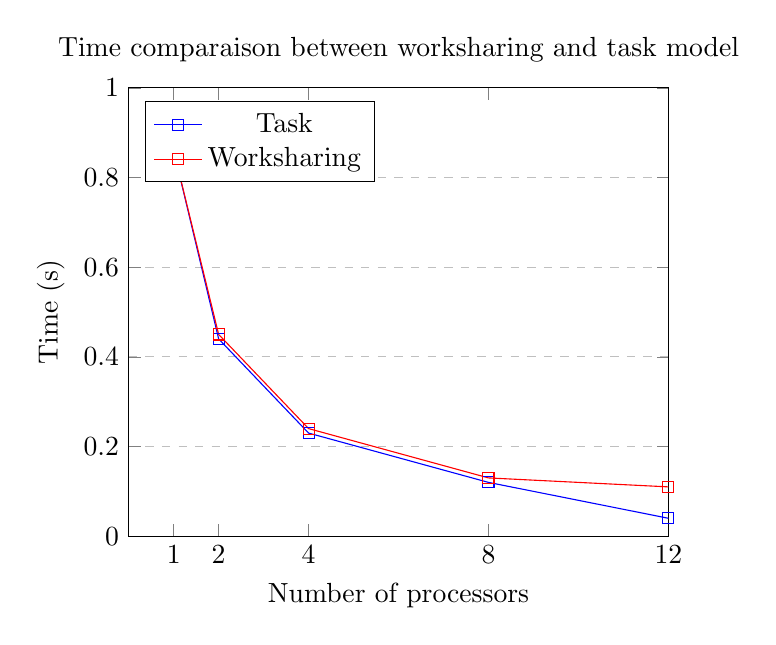
\begin{tikzpicture}
\begin{axis}[
    title={Time comparaison between worksharing and task model},
    xlabel={Number of processors},
    ylabel={Time (s)},
    xmin=0, xmax=12,
    ymin=0, ymax=1,
    xtick={1,2,4,8,12},
    ytick={1,0.8,0.6,0.4,0.2,0},
    legend pos=north west,
    ymajorgrids=true,
    grid style=dashed,
]
 
\addplot[
    color=blue,
    mark=square,
    ]
    coordinates {
    (1,0.86)(2,0.44)(4,0.23)(8,0.12)(12,0.04)
    };
    \addlegendentry{Task}
 
 \addplot[
    color=red,
    mark=square,
    ]
    coordinates {
    (1,0.86)(2,0.45)(4,0.24)(8,0.13)(12,0.11)
    };
    \addlegendentry{Worksharing}
\end{axis}
\end{tikzpicture}
\justify
In this final comparison we can observe that both versions perform equal until 12 processors, when execution times diverge vastly. This may be due to the worksharing constructs not scaling properly with a large number of processors.